\documentclass[12pt, a4paper]{report}

% --- PAQUETES ESENCIALES ---
\usepackage[utf8]{inputenc}
\usepackage[T1]{fontenc}
\usepackage[spanish, es-tabla]{babel} % Idioma español y renombra "Cuadro" a "Tabla"

% --- MATEMÁTICAS ---
\usepackage{amsmath}
\usepackage{amsfonts}
\usepackage{amssymb}

% --- GRÁFICOS Y DISEÑO ---
\usepackage{graphicx}
\usepackage[margin=2.5cm]{geometry}
\usepackage{setspace}
\onehalfspacing % Interlineado 1.5, obligatorio/estándar. ¡Sin errores de grupo!

% --- ENLACES Y METADATOS ---
\usepackage[hidelinks]{hyperref}
\usepackage[nottoc]{tocbibind} % ¡Esta es la línea mágica!
\begin{document}

% ==========================================
% PORTADA PERSONALIZADA (Según normativa)
% ==========================================
\begin{titlepage}
    \centering

    % Asegúrate de tener logo_recortado.pdf en la misma carpeta
    % Si no lo tienes aún, comenta la siguiente línea poniendo un % delante
    
\includegraphics[width=0.4\textwidth]{./images/logo-cuatricromia.pdf}\par\vspace{1cm}

    {\scshape\LARGE Universidad de Valladolid \par}
    \vspace{0.5cm}
    {\scshape\Large Facultad de Ciencias\par}
    \vspace{2cm}

    {\huge\bfseries Mejora de la Ordenación Circular y Robustez en Transcriptómica Circadiana mediante Métodos basados en CPCA\par}
    \vspace{1.5cm}

    {\Large \textit{Trabajo de Fin de Grado en Estadística}\par}
    \vspace{2cm}

    \begin{minipage}[t]{0.4\textwidth}
        \begin{flushleft} \large
            \emph{Autor:}\\
            \textbf{Samuel Ortega Bustos}
        \end{flushleft}
    \end{minipage}
    ~
    \begin{minipage}[t]{0.5\textwidth}
        \begin{flushright} \large
            \emph{Tutores:} \\
            \textbf{Yolanda Larriba González} \\
            \textbf{Juan Camilo Yepes Borrero}
        \end{flushright}
    \end{minipage}\\[2cm]

    \vfill

    {\large \textbf{Curso Académico 2025-2026} \par}
    \vspace{0.5cm}
    {\large \today \par}
\end{titlepage}

% ==========================================
% RESUMEN / ABSTRACT
% ==========================================
\pagenumbering{roman} % Números romanos para los índices

\begin{abstract}
La estimación de la fase circadiana a partir de datos transcriptómicos representa un reto central en cronobiología, especialmente en estudios humanos donde las etiquetas temporales suelen ser inaccesibles por restricciones éticas o clínicas. El algoritmo CIRCUST, basado en el Análisis de Componentes Principales Circulares (CPCA), ha demostrado ser una herramienta prometedora para la reconstrucción del orden temporal. Sin embargo, su implementación actual carece de la modularidad necesaria y de mecanismos para ajustar covariables o manejar muestreos dispersos.

Este trabajo presenta una re-implementación modular y eficiente de CIRCUST en Python, junto con un refinamiento metodológico profundo. Las mejoras incluyen la integración de ajustes por covariables y una optimización de la ordenación circular para mejorar la inferencia de fase. Además, se ha desarrollado un marco de simulación para evaluar sistemáticamente la robustez del modelo frente a perturbaciones como el ruido y los efectos por lotes. Finalmente, el pipeline mejorado se valida utilizando conjuntos de datos transcriptómicos reales del cerebro humano post-mortem, demostrando una mayor precisión y relevancia biológica.

\textbf{Palabras clave:} Cronobiología, Transcriptómica, Ordenación Circular, CPCA, Python.
\end{abstract}

% (Opcional pero recomendado) Abstract en inglés
\renewcommand{\abstractname}{Abstract}
\begin{abstract}
Estimating circadian phase from transcriptomic data is a central challenge in chronobiology, particularly in human studies where time-of-day labels are often unavailable. The CIRCUST algorithm, based on Circular Principal Component Analysis (CPCA), offers a promising approach for temporal order reconstruction. However, its current implementation lacks modularity, extensibility, and built-in mechanisms to adjust for covariates or to handle sparse sampling patterns.

This project presents a modular and efficient re-implementation of CIRCUST in Python, alongside a deep methodological refinement. Improvements include the integration of covariate adjustments and enhanced circular ordering for better phase inference. Furthermore, a simulation framework is developed to systematically evaluate robustness against perturbations such as noise and batch effects. Finally, the improved pipeline is validated using real post-mortem human brain transcriptomic datasets, demonstrating improved accuracy and biological relevance.

\textbf{Keywords:} Chronobiology, Transcriptomics, Circular Ordering, CPCA, Python.
\end{abstract}

% ==========================================
% ÍNDICES
% ==========================================
\tableofcontents
\newpage
\listoffigures
\newpage
\listoftables
\newpage

% ==========================================
% CUERPO DEL TRABAJO
% ==========================================
\pagenumbering{arabic}

\chapter{Introducción}

\section{Contexto Biológico: El Reloj Circadiano}
\subsection{¿Qué es el sistema circadiano?}
Los ritmos circadianos (del latín \textit{circa diem}, que significa ``alrededor de un día'') son oscilaciones biológicas endógenas con un periodo aproximado de 24 horas. Estos ritmos regulan una vasta cantidad de procesos fisiológicos, metabólicos y conductuales en la inmensa mayoría de los organismos vivos, desde cianobacterias hasta seres humanos.

A nivel molecular, este reloj interno no es un concepto abstracto, sino un mecanismo genético muy bien definido. Está impulsado por una intrincada red de genes y proteínas que interactúan formando un bucle de retroalimentación transcripcional-traduccional (TTFL, por sus siglas en inglés). En los mamíferos, este núcleo oscilatorio (conocido como \textit{core clock}) está compuesto por reguladores positivos, como los factores de transcripción CLOCK y BMAL1, y reguladores negativos, principalmente las familias de proteínas Period (PER) y Cryptochrome (CRY). La interacción cíclica de activación y represión de estos genes tarda aproximadamente 24 horas en completarse, dictando así el ritmo basal de la célula.

\subsection{¿Cómo surge y cómo se sincroniza?}

La vida en la Tierra ha evolucionado bajo una constante inalterable: la rotación del planeta y su continuo ciclo de luz y oscuridad. El reloj circadiano surge como una brillante respuesta evolutiva a esta realidad. En lugar de limitarse a reaccionar cuando sale o se pone el sol, los organismos desarrollaron este mecanismo interno para \textit{anticiparse} a los cambios del entorno. De este modo, el cuerpo puede prepararse de antemano para las horas de mayor actividad y demanda metabólica o, por el contrario, ralentizarse para ahorrar energía durante la fase de descanso nocturno.

En los seres humanos, este sistema funciona como una orquesta perfectamente coordinada. El ``director'' es un reloj maestro central situado en el cerebro (en una pequeña región del hipotálamo llamada núcleo supraquiasmático). Este marcapasos principal recibe información directa de la retina en nuestros ojos, lo que le permite utilizar la luz solar para ajustarse y ``ponerse en hora'' cada mañana.

Una vez sincronizado con el ciclo de luz exterior, el reloj maestro se encarga de dirigir al resto del cuerpo. A través de señales nerviosas y hormonales, coordina y pone en hora a una multitud de ``relojes periféricos'' más pequeños. Estos relojes locales residen en la inmensa mayoría de nuestros órganos y tejidos (como el corazón, el hígado, los pulmones o el tejido adiposo), garantizando que toda nuestra maquinaria biológica funcione al unísono y en el momento óptimo del día.

\subsection{¿Por qué es de interés biomédico y clínico?}
La relevancia del reloj circadiano en la transcriptómica moderna es inmensa. Gracias a las tecnologías de secuenciación de alto rendimiento, hoy sabemos que la expresión de una gran proporción del genoma (hasta un 40-50\% dependiendo del tejido) está bajo control circadiano, lo que significa que la actividad de nuestras células cambia drásticamente dependiendo de la hora del día.

Este fenómeno tiene dos implicaciones críticas que justifican el interés científico:
\begin{enumerate}
    \item \textbf{Salud y Patología:} La desalineación crónica del reloj circadiano provocada por factores modernos como el trabajo por turnos (\textit{shift work}), el \textit{jet lag} social, o la exposición nocturna a luz artificial está fuertemente correlacionada con el desarrollo de enfermedades graves. La alteración de los ritmos moleculares es un factor de riesgo comprobado para trastornos metabólicos (diabetes tipo 2, obesidad), enfermedades cardiovasculares, trastornos neurodegenerativos y diversos tipos de cáncer.
    \item \textbf{Cronofarmacología:} Dado que miles de genes fluctúan diariamente, las dianas terapéuticas de muchos fármacos no están igualmente disponibles a todas horas. La eficacia y la toxicidad de un gran número de medicamentos dependen del momento del día en que se administran.
\end{enumerate}

\subsection{El problema de la inferencia del tiempo interno}
El reconocimiento de la profunda influencia del reloj circadiano exige que la investigación biomédica incorpore la variable temporal en sus estudios. En modelos animales, es posible extraer tejidos a intervalos de tiempo estrictamente controlados a lo largo del día. Sin embargo, en estudios transcriptómicos humanos a gran escala (utilizando biopsias clínicas o bases de datos de tejido post-mortem), la hora de extracción es a menudo aleatoria, inexacta o desconocida debido a limitaciones logísticas y éticas.

Aún más problemático es el hecho de que la hora del reloj externo no siempre coincide con el tiempo circadiano interno del individuo, debido a variaciones interpersonales o patologías. Esta ausencia de ``etiquetas temporales'' fiables crea un cuello de botella computacional: ¿cómo podemos estudiar el ritmo de los genes si no sabemos en qué fase del reloj se encontraba la muestra en el momento de la extracción? Es aquí donde surge la necesidad imperiosa de desarrollar metodologías estadísticas avanzadas, capaces de reconstruir el orden temporal de forma latente a partir de los propios datos de expresión génica.
\section{El Problema Fundamental: La Ausencia de Etiquetas Temporales}
Históricamente, el estudio de los ritmos moleculares se ha basado en modelos animales (como ratones) o en ensayos clínicos altamente controlados, donde las muestras se extraen a intervalos de tiempo estrictamente documentados. En estos escenarios, el tiempo de la toma de muestra (etiqueta temporal) es conocido y puede ser utilizado como variable independiente en los modelos estadísticos para identificar qué genes son rítmicos.

Sin embargo, trasladar estos estudios a humanos presenta un desafío monumental. En muchas investigaciones clínicas, especialmente aquellas que utilizan muestras de tejidos u órganos internos (como el tejido cerebral post-mortem de bases de datos como GTEx), la toma de muestras es puramente oportunista. En estos casos, las etiquetas de tiempo exactas (time-of-day o time-of-death) a menudo son inexactas o están completamente ausentes debido a restricciones éticas, logísticas o clínicas.

Incluso cuando se dispone de la hora del reloj en la que se tomó la muestra, esta puede no corresponder con el ``tiempo circadiano interno'' del individuo, el cual puede estar desfasado por factores como el trabajo por turnos, el estilo de vida o la enfermedad.

\section{Inferencia de Fase y Métodos Computacionales Actuales}

Ante la ausencia de etiquetas temporales precisas en los estudios transcriptómicos humanos, la biología computacional ha desarrollado algoritmos capaces de deducir la ``hora interna'' o fase circadiana de cada muestra basándose exclusivamente en el patrón de expresión de sus genes. El principio matemático subyacente de estos métodos consiste en proyectar los datos de alta dimensionalidad (miles de genes evaluados en múltiples muestras) hacia un espacio de menor dimensión que represente geométricamente el ciclo de 24 horas, es decir, una trayectoria cerrada o círculo.

A lo largo de los últimos años, han surgido diversas propuestas algorítmicas para resolver este problema, variando desde técnicas puras de estadística multivariante hasta complejas arquitecturas de aprendizaje automático (\textit{Machine Learning}).

\subsection{CIRCUST: Reconstrucción mediante CPCA y el Modelo FMM}
Entre los enfoques analíticos recientes destaca el algoritmo CIRCUST \cite{larriba2023}, una metodología robusta diseñada para la reconstrucción del orden temporal de los ritmos moleculares. El núcleo matemático de CIRCUST se aleja de las cajas negras y confía en una base estadística transparente y modular, dividiéndose en dos grandes procesos funcionales:

\begin{enumerate}
    \item \textbf{Análisis de Componentes Principales Circulares (CPCA):} En un primer paso, CIRCUST selecciona un subconjunto de ``genes reloj'' centrales y aplica técnicas de reducción de dimensionalidad basadas en CPCA\cite{scholz2007}. Al extraer los dos primeros componentes principales, el algoritmo proyecta las muestras sobre el plano bidimensional delimitado por el círculo unidad. Esto proporciona un orden circular preliminar relativo entre todas las muestras.


    \item \textbf{Aplicación del Modelo FMM:} Una vez establecido el orden circular preliminar de las muestras, CIRCUST emplea el modelo FMM (\textit{Frequency Modulated Möbius})\cite{fmmAlgorithm}. A diferencia de los modelos armónicos clásicos (como las curvas cosenoidales simples), el FMM es un modelo paramétrico no lineal altamente flexible. Esta flexibilidad le permite ajustarse a curvas de expresión génica asimétricas y con formas de onda complejas, logrando una estimación robusta y biológicamente mucho más realista de los componentes oscilatorios.
\end{enumerate}

\subsection{Alternativas Computacionales}
En paralelo a los métodos fundamentados en la estadística clásica, han ganado gran tracción las aproximaciones basadas en \textit{Machine Learning}, destacando particularmente el algoritmo \textbf{CYCLOPS} (\textit{CYclic Ordering by Periodic Structure})\cite{CYCLOPS} y su evolución, CYCLOPS 2.0\cite{CYCLOPS2}.

CYCLOPS representa un cambio de paradigma al delegar la reducción de dimensionalidad en redes neuronales artificiales, específicamente mediante el uso de \textit{autoencoders}. Sus características principales incluyen:

\begin{itemize}
    \item \textbf{Cuello de Botella Circular (\textit{Circular Bottleneck Autoencoder}):} Un autoencoder estándar comprime los datos de entrada en un espacio latente lineal para luego intentar reconstruirlos. La innovación fundamental de CYCLOPS es forzar a la red neuronal a comprimir toda la varianza rítmica de la expresión génica en un espacio latente compuesto por un único nodo circular (una fase que va de 0 a $2\pi$).
    \begin{figure}[htbp]
    \centering
    % Cambia "autoencoder.pdf" por el nombre real de tu archivo de imagen
    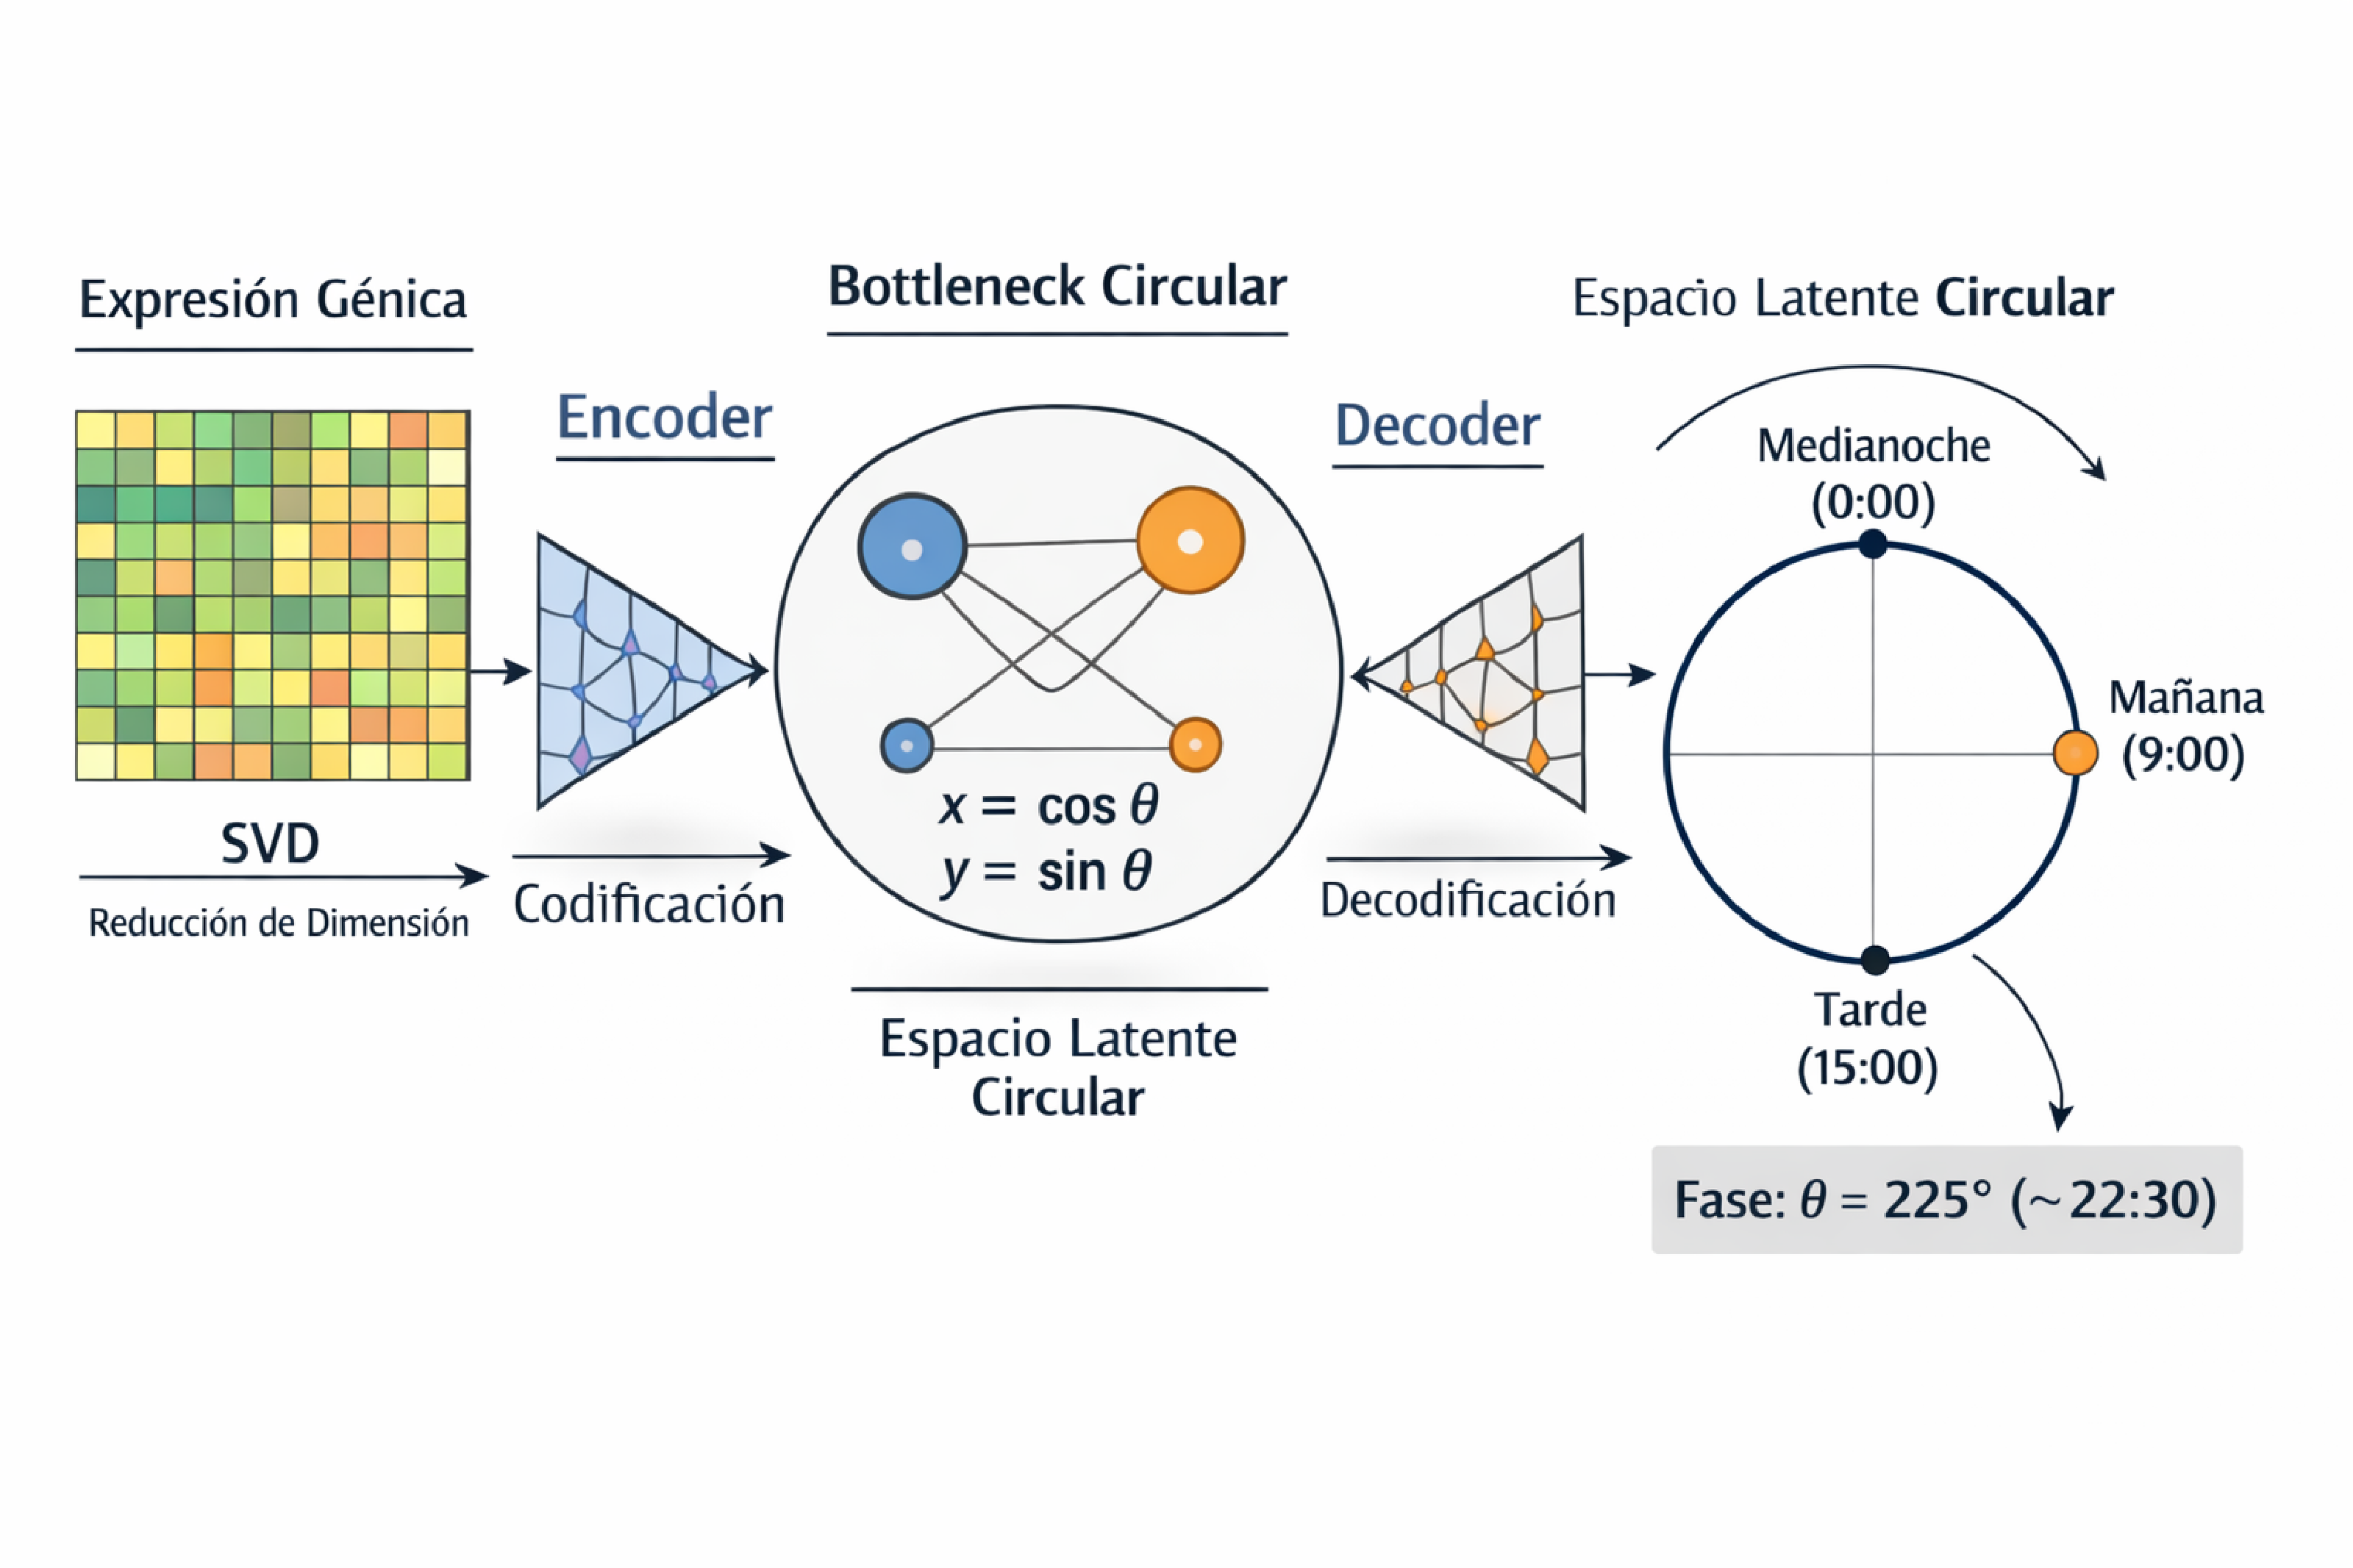
\includegraphics[width=0.8\textwidth]{./images/imagenAutoencoder.pdf}
    \caption{Arquitectura resumida del autoencoder aplicado en CYCLOPS}
    \label{fig:autoencoder}
\end{figure}

    \item \textbf{Corrección de Covariables mediante Codificación Multi-hot:}En datos reales de expresión génica, es habitual que aparezcan variaciones que no están relacionadas con los ritmos circadianos, como diferencias entre tejidos, efectos del laboratorio o características de los pacientes. Estas variaciones pueden ocultar la señal biológica que se quiere estudiar. CYCLOPS 2.0 \cite{CYCLOPS2} introduce una mejora que envuelve al autoencoder original sin modificar su funcionamiento interno. Para ello, utiliza una codificación \textit{multi-hot} que indica qué covariables afectan a cada muestra. Con esta información, el modelo ajusta los datos de entrada para reducir el impacto de esos factores externos antes de comprimir la información en el espacio latente circular.
    Después de reconstruir los datos, se revierte ese ajuste para mantener la coherencia con los valores originales. De esta forma, el modelo consigue centrarse mejor en la señal rítmica de interés y estimar con mayor precisión la fase circadiana, incluso cuando los datos están afectados por ruido o sesgos experimentales.
\end{itemize}
El campo de la inferencia de fase circadiana es sumamente dinámico. Más allá de las dos familias principales representadas por CIRCUST y CYCLOPS, han surgido recientemente otras metodologías computacionales orientadas a resolver desafíos específicos en la reconstrucción del orden temporal:
\begin{itemize}
    \item \textbf{PENN (\textit{Phase Estimation Neural Network}):} parte de la misma idea que CYCLOPS, usar un autoencoder con una capa intermedia circular para asignar a cada muestra una fase angular, sin necesidad de conocer la hora real de recolección. La novedad está en cómo entrena la red. Mientras que un autoencoder convencional solo se preocupa por que la salida se parezca a la entrada (error de reconstrucción), PENN \cite{penn2023} añade un segundo objetivo: que los valores de los genes (o de los componentes principales) sigan una curva cosenoidal cuando se ordenan según la fase estimada. En términos sencillos, la red aprende a organizar las muestras en el ciclo circadiano de manera que la expresión de cada gen se ajuste a una onda periódica, al mismo tiempo que conserva la estructura global de los datos. Esta regularización estabiliza la estimación y la hace más robusta frente al ruido propio de los datos biológicos, mostrando mejoras respecto a CYCLOPS en los conjuntos evaluados.
    \item \textbf{CHIRAL:} Es un algoritmo matemático diseñado específicamente para abordar el desafío de los conjuntos de datos transcriptómicos multi-tejido (como datos del consorcio GTEx). En lugar de tratar todos los tejidos como un solo bloque, CHIRAL \cite{chiral2020} opera jerárquicamente. Primero, estima una Fase Interna del Tejido (TIP, por sus siglas en inglés) independiente para cada órgano utilizando genes reloj específicos. Posteriormente, integra las fases de todos los tejidos pertenecientes a un mismo individuo post-mortem para inferir una Fase Interna del Donante (DIP) global y consolidada. Este enfoque permite separar la variabilidad entre tejidos de la fase circadiana sistémica del individuo, mejorando la coherencia temporal en estudios transcriptómicos a gran escala.
\end{itemize}
Si bien enfoques como CYCLOPS ofrecen una gran capacidad para modelar relaciones no lineales en datos complejos, la naturaleza opaca de las redes neuronales dificulta la interpretabilidad rigurosa de los resultados. En este contexto, la reimplementación y mejora de métodos transparentes basados en componentes principales, como CIRCUST, resulta especialmente valiosa.
\section{Limitaciones Existentes y Motivación del Trabajo}

Para comprender la necesidad de optimizar las herramientas algorítmicas en cronobiología, es imprescindible analizar primero las severas restricciones del entorno de datos en el que operan estos modelos, así como las debilidades metodológicas presentes en el estado de los modelos actuales.

\subsection{El Cuello de Botella de los Datos: La Dependencia de GTEx}
El mayor obstáculo en el estudio de los ritmos circadianos humanos a nivel transcriptómico es la recolección de muestras. Obtener series temporales en vivo de órganos internos (como el cerebro, el corazón o el hígado) mediante biopsias repetidas a lo largo de 24 horas es ética, clínica y logísticamente inviable debido a los altos riesgos para el paciente. 

Como consecuencia, la investigación moderna depende de donaciones de tejido post-mortem. En este contexto, el proyecto \textbf{GTEx (\textit{Genotype-Tissue Expression})} \cite{gtex2020} se ha consolidado como la base de datos de referencia mundial, proporcionando un atlas masivo de expresión génica en múltiples tejidos humanos. Sin embargo, el uso de cohortes post-mortem como GTEx introduce un nivel de ruido estadístico extremo: cada donante aporta una única muestra por tejido (un solo punto en el tiempo), la hora exacta de la muerte (\textit{time of death}) suele ser imprecisa, y existen variables de confusión inevitables como el tiempo de isquemia\footnote{En transcriptómica post-mortem, el tiempo de isquemia se refiere al intervalo transcurrido desde la interrupción del flujo sanguíneo (fallecimiento) hasta la estabilización o congelación de la muestra. Durante este periodo, la degradación del ARN y la respuesta celular a la hipoxia alteran significativamente los perfiles de expresión génica, introduciendo sesgos severos en el análisis.}, la causa de la muerte o el tiempo transcurrido hasta la preservación del tejido. Inferir un reloj circadiano continuo a partir de estas ``fotografías aisladas'' es el verdadero reto.

\subsection{Limitaciones en las Alternativas Computacionales}
Aunque metodologías avanzadas como CYCLOPS, PENN o CHIRAL han intentado resolver este rompecabezas, todas presentan compromisos algorítmicos (\textit{trade-offs}) que limitan su aplicabilidad universal:

\begin{itemize}
    \item \textbf{Opacidad y Dependencia de Datos (CYCLOPS y PENN):} Al basarse en arquitecturas de redes neuronales profundas (\textit{Deep Learning}), estos métodos actúan como ``cajas negras''. Aunque la codificación \textit{multi-hot} de CYCLOPS 2.0 y la función de coste híbrida de PENN son matemáticamente sofisticadas, carecen de una trazabilidad estadística estricta. Además, las redes neuronales son propensas al sobreajuste (\textit{overfitting}) cuando se enfrentan a conjuntos de datos con un número de muestras reducido (un problema crónico en transcriptómica), requiriendo un ajuste intensivo de hiperparámetros.
    \item \textbf{Suposiciones Estructurales Rígidas (CHIRAL):} Métodos como CHIRAL fueron diseñados ad-hoc para infraestructuras multi-tejido masivas como GTEx. Su efectividad disminuye significativamente cuando se aplican a estudios clínicos más pequeños o de un solo tejido, al depender de la jerarquía estadística entre los diferentes órganos del mismo donante para estabilizar su inferencia.
\end{itemize}

\subsection{Limitaciones Específicas de CIRCUST}
Frente a los modelos de caja negra, CIRCUST \cite{larriba2023} ofrece una solución basada en estadística clásica (CPCA y modelo FMM) que garantiza interpretabilidad geométrica y biológica. No obstante, la implementación actual del algoritmo presenta debilidades críticas, tanto teóricas como de ingeniería de software, que restringen su adopción clínica:

\begin{enumerate}
    \item \textbf{Vulnerabilidad ante Factores de Confusión (Covariables):} Esta es la limitación estadística más grave. La formulación matemática original de CIRCUST asume que toda la varianza cíclica capturada en los dos primeros Componentes Principales se debe exclusivamente a la señal del reloj biológico. El algoritmo no posee un mecanismo interno para filtrar el ruido introducido por efectos de lote (\textit{batch effects}), el sexo, la edad o patologías subyacentes. Si no se corrigen estos sesgos antes de proyectar las muestras en el círculo unitario, la inferencia de la fase resultará geométricamente deformada.
    \item \textbf{Inestabilidad frente al Muestreo Disperso (\textit{Sparse Sampling}):} La precisión de la estimación del orden circular mediante CPCA decae abruptamente si la distribución temporal real de las muestras (por ejemplo, en cohortes donde la mayoría de los decesos ocurren en una misma franja horaria) presenta grandes huecos o no es uniforme a lo largo del ciclo de 24 horas.
\item \textbf{Rigidez Arquitectónica y Ausencia de Modularidad:} Aunque R es el ecosistema de referencia para el desarrollo de software estadístico en bioinformática, la implementación original de CIRCUST se concibió como un \textit{script} procedimental y monolítico. Esta falta de estructura modular dificulta su integración transparente en \textit{pipelines} de análisis de datos más complejos o híbridos (especialmente aquellos que combinan estadística clásica con \textit{Machine Learning} en ecosistemas Python). Además, esta rigidez de código impide aislar, probar y sustituir fácilmente componentes matemáticos concretos para la experimentación metodológica, penalizando la eficiencia y la capacidad de paralelización cuando se requiere ejecutar simulaciones sintéticas a gran escala.
\end{enumerate}

\subsection{Motivación y Justificación del Trabajo}
La convergencia de estas problemáticas motiva directamente el desarrollo de este Trabajo de Fin de Grado. El objetivo central no es simplemente la traducción de código de R a Python, sino una \textbf{re-arquitectura integral y un refinamiento estadístico profundo de la metodología CIRCUST}. 

En particular, la incorporación de mecanismos de corrección de covariables mediante \textbf{regresión lineal sobre los componentes principales} permitirá aislar matemáticamente la señal rítmica del ruido del entorno (resolviendo el problema de los efectos de lote en datos como GTEx). Al combinar esta corrección interpretable con una nueva implementación modular, eficiente y paralelizable en Python, este trabajo dotará a CIRCUST de la robustez necesaria para procesar conjuntos de datos biológicos ruidosos y heterogéneos, acercando el rendimiento estadístico transparente al de los complejos modelos de aprendizaje profundo sin sacrificar su interpretabilidad.

\chapter{Objetivos}
El propósito fundamental de este trabajo es la re-implementación y el refinamiento metodológico del algoritmo CIRCUST, dotándolo de una arquitectura de software moderna y mejorando su solidez estadística. Para alcanzar este propósito, se establecen los siguientes objetivos específicos:

\begin{enumerate}
    \item \textbf{Re-implementación Modular en Python:} Migrar y reestructurar el código original de CIRCUST hacia un entorno Python orientado a objetos. Esto garantizará la extensibilidad del software, facilitando su integración en pipelines computacionales más amplios y mejorando su eficiencia algorítmica.
    \item \textbf{Refinamiento de la Inferencia de Fase y Ajuste de Covariables:} Mejorar la precisión de la ordenación circular mediante la integración de modelos de regresión que permitan corregir los componentes principales en función de covariables clínicas o técnicas, aislado así la señal puramente circadiana.
\end{enumerate}

\chapter{Metodología Matemática}
% Aquí introduciremos las bases matemáticas de CPCA y el modelo FMM.
(En desarrollo...)

\chapter{Diseño e Implementación en Python}
% Aquí detallaremos la arquitectura modular: módulos de preprocesamiento, inferencia y validación.
(En desarrollo...)

\chapter{Resultados y Simulaciones}
% Análisis de la comparación entre la versión original y la nueva, resultados con ruido y datos GTEx.
(En desarrollo...)

\chapter{Conclusiones y Trabajo Futuro}
% Resumen de logros. Si da tiempo, mención a la comparativa con CYCLOPS 2.0.
(En desarrollo...)

% ==========================================
% BIBLIOGRAFÍA
% ==========================================
\begin{thebibliography}{9}

\bibitem{larriba2023}
Larriba, Y., Mason, I. C., Saxena, R., Scheer, F. A. J. L., y Rueda, C. (2023).
\textit{CIRCUST: A novel methodology for temporal order reconstruction of molecular rhythms; validation and application towards a daily rhythm gene expression atlas in humans}.
PLOS Computational Biology, 19(9):e1011510. \url{https://doi.org/10.1371/journal.pcbi.1011510}

\bibitem{scholz2007}
Scholz, M. (2007).
\textit{Analysing periodic phenomena by circular pca}.
En \textit{Bioinformatics Research and Development (BIRD 2007)} (pp. 38-47). Springer.

\bibitem{CYCLOPS}
Anafi, R., Francey, L., Hogenesch, J., y Kim, J. (2017).
\textit{CYCLOPS reveals human transcriptional rhythms in health and disease}.
Proceedings of the National Academy of Sciences of the United States of America, 114(20):5312--5317. \url{https://doi.org/10.1073/pnas.1619320114}

\bibitem{CYCLOPS2}
Hammarlund, J. A. (2025).
\textit{CYCLOPS 2.0: improving and applying circadian phase reconstruction in confounded datasets} (Tesis doctoral).
Drexel University, Filadelfia, Pensilvania.

\bibitem{penn2023}
Seyed, M. A., et al. (2023).
\textit{PENN: Phase Estimation Neural Network on Gene Expression Data}.
En \textit{Bioinformatics and Biomedicine}. \url{https://doi.org/10.1007/978-3-031-39821-6_1}

\bibitem{chiral2020}
Talamanca, L., et al. (2023).
\textit{Sex-dimorphic and age-dependent organization of 24-hour gene expression rhythms in humans}.
Science, 379(6631):478-483. \url{https://doi.org/10.1126/science.add0846}
% (Nota: Talamanca et al. son los creadores y máximos exponentes del uso del algoritmo CHIRAL sobre los datos del GTEx).

\bibitem{fmmAlgorithm}
Rueda, C., Larriba, Y., y Peddada, S. (2019).
\textit{Frequency Modulated Möbius Model Accurately Predicts Rhythmic Signals in Biological and Physical Sciences}.
Scientific Reports, 9:18701. \url{https://doi.org/10.1038/s41598-019-54569-1}

\bibitem{gtex2020}
GTEx Consortium (2020). 
\textit{The GTEx Consortium atlas of genetic regulatory effects across human tissues}. 
Science, 369(6509):1318-1330. \url{https://doi.org/10.1126/science.aaz1776}

\end{thebibliography}

\end{document}
